%------------ Configuração Completa ------------%
\documentclass[11pt]{beamer}
\usetheme{Darmstadt}

%------------ Pacotes ------------%
\usepackage[utf8]{inputenc}
\usepackage[brazilian]{babel}
\usepackage[T1]{fontenc}
\usepackage{amsmath}
\usepackage{amsfonts}
\usepackage{amssymb}
\usepackage{graphicx}
\usepackage{xcolor} 
\usepackage{tikz}
\usepackage{tabularx}
\usepackage{makecell}
\usepackage{setspace}
\usepackage{adjustbox}
\usepackage{makecell}
\usepackage{caption}
\usepackage{float}
\usepackage{graphicx}
\usepackage{multirow}
\usepackage{pdflscape}
\usepackage{booktabs}
\usepackage[ruled,vlined]{algorithm2e}

% ----------- Config. tikz ------------- %
\usetikzlibrary{shapes.geometric, arrows, positioning, shadows}

% ----------- Personalizados ------------- %
\newcommand{\fonte}[1]{%
    \par
    \raggedright
    {Fonte: #1}
}

\renewcommand{\algorithmcfname}{Algoritmo}
\SetKwInput{KwIn}{Entrada}
\SetKwInput{KwOut}{Saída}
\SetKwFor{Para}{para}{faça}{fim para}
\SetKwIF{Se}{SenaoSe}{Senao}{se}{então}{senão se}{senão}{fim se}

% -------------------------------------- %

% Configuração específica para tabelas/quadros
\def\tablename{Quadro}
\DeclareCaptionLabelSeparator{hyphen}{ - }

% Configura todas as legendas do documento para usar o novo estilo
\captionsetup{labelsep=hyphen, justification=centering, font=bf, skip=0pt}


%------------ Definição de cor ------------%
\definecolor{myblue}{RGB}{48, 48, 171}

%------------ Comandos e Templates ------------%
\DeclareMathOperator{\sen}{sen}
\DeclareMathOperator{\tg}{tg}
\setbeamertemplate{caption}[numbered]
\setbeamertemplate{navigation symbols}{} 
\bibliographystyle{apalike}

%------------ Informações do Documento ------------%
\title{Impacto Da Aplicação Dos Critérios Mínimos Para Seleção De Tábuas De Mortalidade Sobre As Provisões Matemáticas Dos Regimes Próprios De Previdência Social}

\author[Stênio]{Aluno: João Pedro Stênio Farias da Silva \\ Orientador: Prof. Me. Yuri Martí Santana Santos \\ Coorientador: Prof. Dr. Luiz Carlos Santos Júnior \\ 1º Avaliador: Prof. Bel. Hugo Vieira Sá Ferreira Gomes \\ 2º Avaliador: Profa. Dra. Everlane Suane de Araújo da Silva}

\institute[]{Universidade Federal da Paraíba \par Centro de Ciências Sociais Aplicadas \par Departamento de Finanças e Contabilidade \par Graduação em Ciências Atuariais} 

\date{João Pessoa - 2026} 

%------------ Logo UFPB ------------%
\logo{
\includegraphics[height=1cm]{logo-ufpb.png}}


\begin{document}

%------------ Frame de Título ------------%
\begin{frame}
    \begin{center}
        % 1. Instituição
        {\small \insertinstitute}
        \vfill
        
        % Título estilizado como na imagem
        \begin{tikzpicture}
            \node[
                fill=myblue,
                text=white,
                rounded corners=8pt,
                drop shadow,
                text width=0.9\textwidth,
                align=center,
                inner sep=12pt
            ] 
            {\usebeamerfont{title}\inserttitle};
        \end{tikzpicture}
        
        \vfill
        
        % Autores (com fonte diminuída)
        \usebeamerfont{author}{\small\insertauthor}\par
        \vspace{0.2cm}
        
        % Data
        \usebeamerfont{date}\insertdate\par
    \end{center}
\end{frame}

%------------ Sumário ------------%
\begin{frame}{Sumário}
    \tableofcontents 
\end{frame}

%------------ Capítulo 1 ------------%
\section{Introdução e Problema}
    
    %------------ Tela para introdução e contextualização ------------%
    \begin{frame}

        %------------ Título do slide ------------%
        \frametitle{Introdução e Contextualização}

        %------------ Primeiro tópico ------------%
        \begin{itemize}
            
            \item \textbf{Regimes Próprios de Previdência Social (RPPS)}

        %------------ Espaço entre tópicos ------------%
        \medskip

        %------------ Segundo tópico ------------%
        \item \textbf{Sustentabilidade}

            %------------ Subtópicos ------------%
            \begin{itemize}
            
                \item[-] Equilíbrio Financeiro
                \medskip
                \item[-] Equilíbrio Atuarial
                
            \end{itemize}

        %------------ Espaço entre tópicos ------------%
        \medskip
        
        %------------ Terceiro tópico ------------%
        \item \textbf{Premissas Atuariais}

            %------------ Subtópicos ------------%
            \begin{itemize}
            
                \item[-] Biométricas
                \medskip
                \item[-] Econômicas
                \medskip
                \item[-] Genéricas
                
            \end{itemize}
            
        %------------ Espaço entre tópicos ------------%
        \medskip
        
        %------------ Quarto tópico ------------%
        \item \textbf{Situação Atual}

            %------------ Subtópicos ------------%
            \begin{itemize}
                \item[-] Em 2021 os RPPS somaram cerca de R\$ 2,5 trilhões déficit atuarial.
            \end{itemize}
    
        \end{itemize}
        
    %------------ Final da introdução e contextualização ------------%   
    \end{frame}
    

    %------------ Tela para o problema ------------%
    \begin{frame}

        %------------ Título do slide ------------%
        \frametitle{Problema}

        \begin{itemize}

            %------------ Primeiro tópico ------------%
            \item \textbf{Portaria MTP Nº 1.467/2022}
        
            \medskip

            %------------ Segundo tópico ------------%
            \item \textbf{Art. 36, inciso I, da Seção VI, Capítulo IV}

                %------------ Subtópicos ------------%
                \begin{itemize}
                    \item[(a)] Será dado pela tábua anual de mortalidade do Instituto Brasileiro de Geografia e Estatísticas - IBGE, segregada obrigatoriamente por sexo, divulgada pela SPREV;
            
                    \item[(b)] Será averiguado por meio da comparação entre a Expectativa de Vida - Ex estimada por essa tábua com aquela gerada pelas tábuas utilizadas na avaliação atuarial, com base na idade média geral da massa de segurados do RPPS.
                    
                \end{itemize}

            \medskip

            %------------ Terceiro tópico ------------%
            \item \textbf{Escolha da média como ponto de avaliação}
            \item \textbf{Escolha de $e_{\overline{X}}$ como única medida}

            
        \end{itemize}
        
    %------------ Fim da tela para o problema ------------%
    \end{frame}

    %------------ Tela para o problema ------------%
    \begin{frame}

        %------------ Título do slide ------------%
        \frametitle{Problema}

        \begin{itemize}
            \item Interpretação do referido artigo
            
            \begin{itemize}
                \item[-] $e^{*}_{\overline{X}} \geq e^{r}_{\overline{X}} \Rightarrow PM^{*} \geq PM^{r}$
            \end{itemize}

            \medskip

            \item Simplificando a impliação
            \begin{itemize}
                \item[-] $e^{*}_{x} \geq e^{r}_{x} \Rightarrow a^{*}_{x} \geq a^{r}_{x}$
            \end{itemize}
            
            \medskip
            
            \item $e_{x} = \sum_{t=1}^{\omega-x} {}_{t}p_{x} = \mathbf{1}^\top \mathbf{p}_x$
            
            \item $a_{x} = \sum_{t=1}^{\omega-x} v^{t}\cdot {}_{t}p_{x} = \mathbf{v}^\top \mathbf{p}_x$
            
            \medskip

        \end{itemize}
        
    %------------ Fim da tela para o problema ------------%
    \end{frame}

    %------------ Tela para o problema ------------%
    \begin{frame}

        \frametitle{Problema}

            \begin{table}
            \centering
            \caption{Exemplo numérico}
                \begin{tabular}{c|c} \hline
                \textbf{Tábua comparativa $*$} & \textbf{Tábua de referência $r$} \\ \hline

                ${}_{1}p^{*}_x = 0{,}6447$ & ${}_{1}p^{r}_x = 0{,}8915$ \\

                ${}_{2}p^{*}_x = 0{,}5600$ & ${}_{2}p^{r}_x = 0{,}4187$ \\

                ${}_{3}p^{*}_x = 0{,}1214$ & ${}_{3}p^{r}_x = 0{,}0104$ \\ \hline

                \end{tabular}
                \vspace{0.25cm}
                \fonte{Elaboração própria (2026).}
            \end{table}
            
            \begin{center}
                \fbox{
                $e^{*}_{x} = 1{,}3261$, $e^{r}_{x} = 1{,}3205$, 
                $a^{*}_{x} = 1{,}2268$ e $a^{r}_{x} = 1{,}2377$
                }
            \end{center}
            
            \begin{center}
                \fbox{
                $e^{*}_{x} \geq e^{r}_{x}$, 
                $a^{*}_{x} < a^{r}_{x}$
                }
            \end{center}
    \end{frame}
    
    %------------ Tela para a pergunta de pesquisa ------------%
    \begin{frame}
        
        %------------ Título do slide ------------%
        \frametitle{Pergunta de Pesquisa}

            %------------ Bloco com a pergunta de pesquisa ------------%
            \begin{alertblock}{Pergunta Central da Pesquisa}
                Qual o impacto da aplicação dos critérios mínimos para a seleção de tábuas de vida — conforme o Art. 36 da Portaria MTP Nº 1.467/2022 — sobre as provisões matemáticas?
            \end{alertblock}

    %------------ Fim da tela para a pergunta de pesquisa ------------%
    \end{frame}

    %------------ Tela objetivo geral ------------%
    \begin{frame}

        %------------ Título do slide ------------%
        \frametitle{Objetivo Geral}

        \textbf{Este estudo propõe-se a analisar o impacto da aplicação dos critérios mínimos para a seleção de tábuas de vida - conforme o Art. 36 da Portaria MTP Nº 1.467/2022 - sobre as provisões matemáticas.}

    %------------ Fim da tela objetivo geral ------------%
    \end{frame}
    
    %------------ Tela objetivos específicos ------------%
    \begin{frame}

        %------------ Título do slide ------------%
        \frametitle{Objetivos Específicos}

            %------------ Tópicos ------------%
            \begin{enumerate}
                \item Realização de simulações computacionais para quatro perfis etários distintos.

                \item Calcular as provisões matemáticas para cada perfil simulado, considerando os métodos de custeio INE, CUP e PNI para as tábuas selecionadas.
                
                \item Identificar as tábuas de mortalidade que, embora atendam ao critério normativo, resultem em provisão matemática inferior à gerada pela tábua de referência.
                
                \item Investigar as causas desses resultados e propor um indicador que permita suspeitar se uma tábua poderá gerar uma provisão matemática inferior àquela obtida pela tábua de referência.

            \end{enumerate}

    %------------ Fim da tela objetivos específicos ------------%
    \end{frame}

        %------------ Tela da justificativas ------------%
    \begin{frame}

        %------------ Título do slide ------------%
        \frametitle{Justificativa}

            %------------ Tópicos ------------%

            \textbf{Verificação da aplicabilidade do Art. 36}
                %------------ Subtópicos ------------%
                \begin{itemize}
                    \medskip
                    \item Simplifica a validação de um fenômeno complexo e distribucional.
                \end{itemize}
            
            \bigskip

            \textbf{Estudo de Rocha \textit{et al} (2024)}
            
            \bigskip

            \textbf{No execício de 2025 aproximadamente 50\% dos RPPS não utilizaram a tábua mínima para a população masculina e mesma proporção para a população feminina}

    %------------ Fim da tela da justificativas ------------%
    \end{frame}

%------------ Capítulo 2 ------------%
\section{Referencial Teórico}

    %------------ Tela para referencial teórico ------------%
    \begin{frame}

        %------------ Título do slide ------------%
        \frametitle{Referencial Teórico}

            %------------ Primeiro tópico ------------%
            \textbf{Revisão Bibliográfica}

                %------------ Subtópicos ------------%
                \begin{itemize}
                    \item Castro e Silva (2019).
                    \item Gonzaga \textit{et al} (2022).
                    \item Rocha \textit{et al} (2024).
                \end{itemize}

            \bigskip

            %------------ Segundo tópico ------------%
            \textbf{Regulamentação}

                %------------ Subtópico ------------%
                \begin{itemize}
                    \item Emenda Constitucional nº 20/1998.
                    \item Art. 40 da  Constituição Federal.
                    \item Lei nº 9.717, de 27 de novembro de 1998.
                    \item Decreto nº 3.788/2001.
                    \item Portaria MTP Nº 1.467, de 2 de junho de 2022.
                \end{itemize}

    %------------ Fim da tela para o referencial teórico ------------%
    \end{frame}

    %------------ Tela para cálculo atuarial ------------%
    \begin{frame}

        %------------ Título do slide ------------%
        \frametitle{Cálculo Atuarial em Sistemas Previdenciários}

            %------------ Tópico ------------%
            \textbf{Projeção dos fluxos futuros}
                \medskip

                %------------ Subtópicos ------------%
                \begin{itemize}
                    \item Técnicas Financeiras $\to$ Fatores de Desconto Financeiro
                    \medskip
                    \item Técnicas Biométricas $\to$ Tábuas de Mortalidade
                    \bigskip
                    \item Provisões Matemáticas
                        \medskip
                        \begin{itemize}
                            \item[$-$] PMBC
                            \medskip
                            \item[$-$] PMBaC
                        \end{itemize}
                    \item Regimes Financeiros e Métodos de Custeio
                \end{itemize}


    %------------ Fim da tela para cálculo atuarial ------------%
    \end{frame}

%------------ Capítulo 3 ------------%
\section{Metodologia}

    %------------ Tela para tipologia e base de dados ------------%
    \begin{frame}

        %------------ Título do slide ------------%
        \frametitle{Metodologia}

            %------------ Tópico ------------%
            \textbf{Tipologia}
            \medskip

                %------------ Subtópicos ------------%
                \begin{itemize}
                    \item Quantitativa
                    \medskip
                    \item Exploratória
                    \medskip
                    \item Empírico - Aplicado
                \end{itemize}
            \bigskip

            %------------ Tópico ------------%
            \textbf{Base de Dados}
                \medskip

                %------------ Subtópicos ------------%
                \begin{itemize}
                    \item Simulação computacional
                \end{itemize}

    %------------ Fim da tela para tipologia e base de dados ------------%
    \end{frame}

    % --- Tela Pseudocodigo --- %
    \begin{frame}


        %------------ Título do slide ------------%
        \frametitle{Pseudocodigo Tábuas}
        

            \begin{figure}[H]
                \centering
                \resizebox{0.8\linewidth}{!}{
                \begin{minipage}{\linewidth}
                \begin{algorithm}[H]
                    \caption{Procedimento para seleção de tábuas}

                    \KwIn{Base de dados e conjunto de tábuas}
                    \KwOut{Conjunto de tábuas aprovadas}

                    Carregar base de dados\;

                    Calcula-se a idade média geral do grupo\;

                    A base é divida em subconjuntos, um para cada gênero\;

                    \Para{cada gênero}{
                        Busca-se na tábua de referência (IBGE 2024 extrapolada para o gênero) a expectativa de vida na idade média do grupo\;

                        \Para{cada tábua comparativa}{
                            Busca-se a expectativa de vida na idade média do grupo\;
                            
                            \eSe{Expectativa de vida da tábua comparativa $\geq$ expectativa da tábua de referência}{
                                Aprovar a tábua para o gênero em análise\;
                            }{
                                Descartar a tábua (não atende ao critério mínimo)\;
                            }
                        }
                    }
                \end{algorithm}
                \end{minipage}
                }
            \end{figure}
    \end{frame}

    %------------ Tela para procedimento de análise ------------%
    \begin{frame}

        %------------ Título do slide ------------%
        \frametitle{Procedimento de Análise}

            %------------ Tópico ------------%
            
            \textbf{Calculo da provisão matemática por três métodos de custeio}

            \bigskip

            \textbf{Análise comparativa e identificação de inconsistências}
            
            \bigskip
            
            \textbf{Investigação de fatores explicativos}
            
            \bigskip
                \begin{itemize}
                    \item Curva de $l_x$
                    \medskip
                    \item Calculo e análise do índice proposto
                    \medskip
                    \begin{itemize}
                        \item[-] $    I_F = \left(\frac{\sum_{f \in F}{} l^{*}_{f} \cdot w(f)}{\sum_{f \in F}{} l^{r}_{f} \cdot w(f)} - 1 \right) \cdot 100$ 
                    \end{itemize}
                \end{itemize}

    %------------ Fim da tela para procedimento de análise ------------%
    \end{frame}


\section{Resultados}

    % --- Tela base de dados simulados --- %
    \begin{frame}

        % --- Título do slide --- %
        \frametitle{Base de dados}

            % --- Figura pirâmides etárias --- %
            \begin{figure}
                \caption{Pirâmides etárias}
                \resizebox{0.775\linewidth}{!}{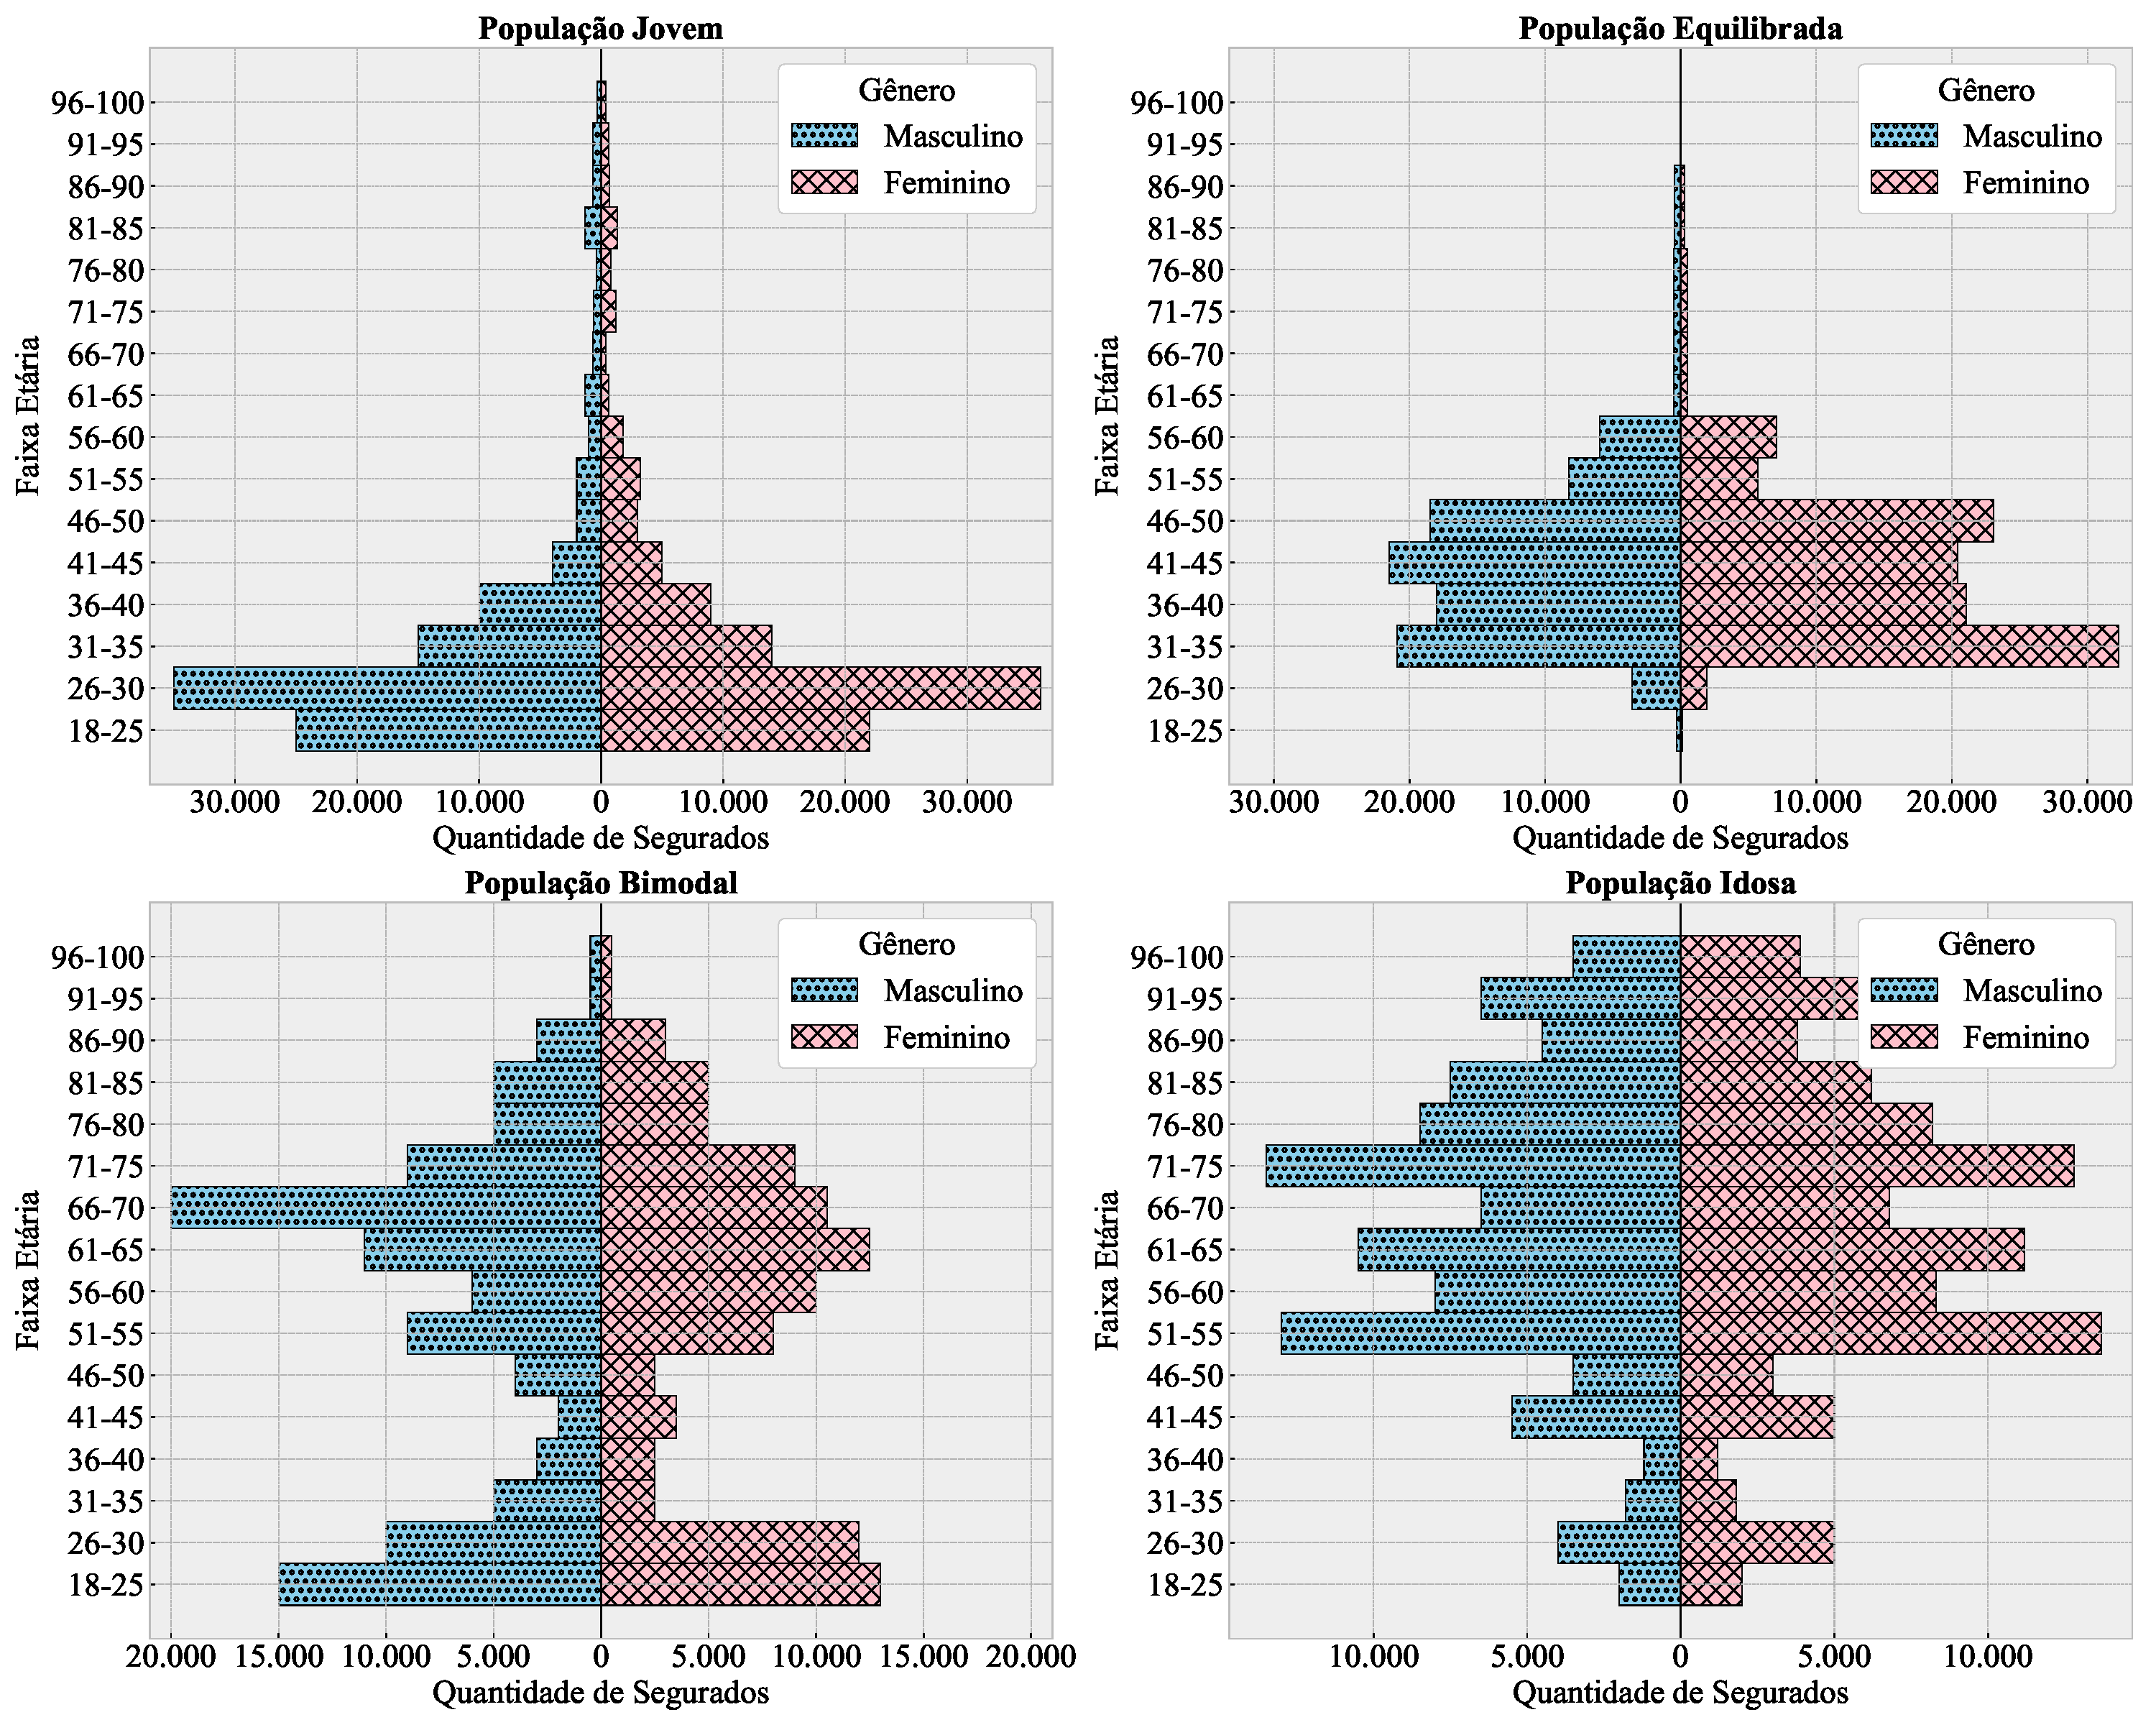
\includegraphics[width=1.0\textwidth, trim=0 0 0 0, clip]{piramides_etarias.pdf}}
            \end{figure}

    % --- Fim tela base de dados simulados --- %
    \end{frame}

    % --- Tela provisões matemáticas --- %
    \begin{frame}

        % --- Título do slide --- %
        \frametitle{Provisões Matemáticas e Inconsistências}

            % --- Tabela com resultados --- %
            \begin{table}[H]
                \centering
                \caption{Número de Tábuas Inconsistentes por Base, Método e Gênero}
                \renewcommand{\arraystretch}{1.1}
                \begin{tabular}{lcccccc}
                \toprule
                & \multicolumn{2}{c}{\textbf{INE}} & \multicolumn{2}{c}{\textbf{CUP}} & \multicolumn{2}{c}{\textbf{PNI}} \\
                \cmidrule(lr){2-3}\cmidrule(lr){4-5}\cmidrule(lr){6-7}
                \textbf{Base} & \textbf{Masc.} & \textbf{Fem.} & \textbf{Masc.} & \textbf{Fem.} & \textbf{Masc.} & \textbf{Fem.} \\
                \midrule
                Jovem       & 10 & 3 & 8 & 3 & 12 & 4 \\
                Equilibrada &  7 & 4 & 6 & 4 &  8 & 5 \\
                Bimodal     &  1 & 1 & 1 & 1 &  5 & 3 \\
                Idosa       &  1 & 1 & 1 & 1 &  5 & 4 \\
                \midrule
                \textbf{Total} & \textbf{19} & \textbf{9} & \textbf{16} & \textbf{9} & \textbf{30} & \textbf{16} \\
                \bottomrule
                \end{tabular}
                \label{tab:sintese_inconsistencias}
                \vspace{0.25cm}
                \fonte{Elaboração própria (2026).}
            \end{table}

    % --- Fim tela provisões matemáticas --- %
    \end{frame}

    % --- Tela pontos de discussão --- %
    \begin{frame}

        % --- Título do slide --- %
        \frametitle{Discussão}

            % --- itens --- %
            \begin{itemize}
                \item Estruturas etárias mais jovens podem estar mais suscetíveis
                \medskip
                \item Inconsistências por método de custeio
                \medskip
                \item Inconsistências por gênero
                \medskip
                \item Suavização/Agravamento de tábuas
            \end{itemize}

    % --- Fim tela pontos de discussão --- %
    \end{frame}

    % --- Tela curva lx masculina --- %
    \begin{frame}
        \frametitle{Curva $l_x$ Masculina}

            \begin{figure}
                \centering
                \caption{$l_x$ Masculino}
                
\includegraphics[width=0.9\textwidth, trim=0 0 0 2.5cm, clip]{curva_lx_masc.pdf}
            \end{figure}
    \end{frame}


    \begin{frame}
        \frametitle{Curva $l_x$ Feminina}

            \begin{figure}
                \centering
                \caption{$l_x$ Feminino}
                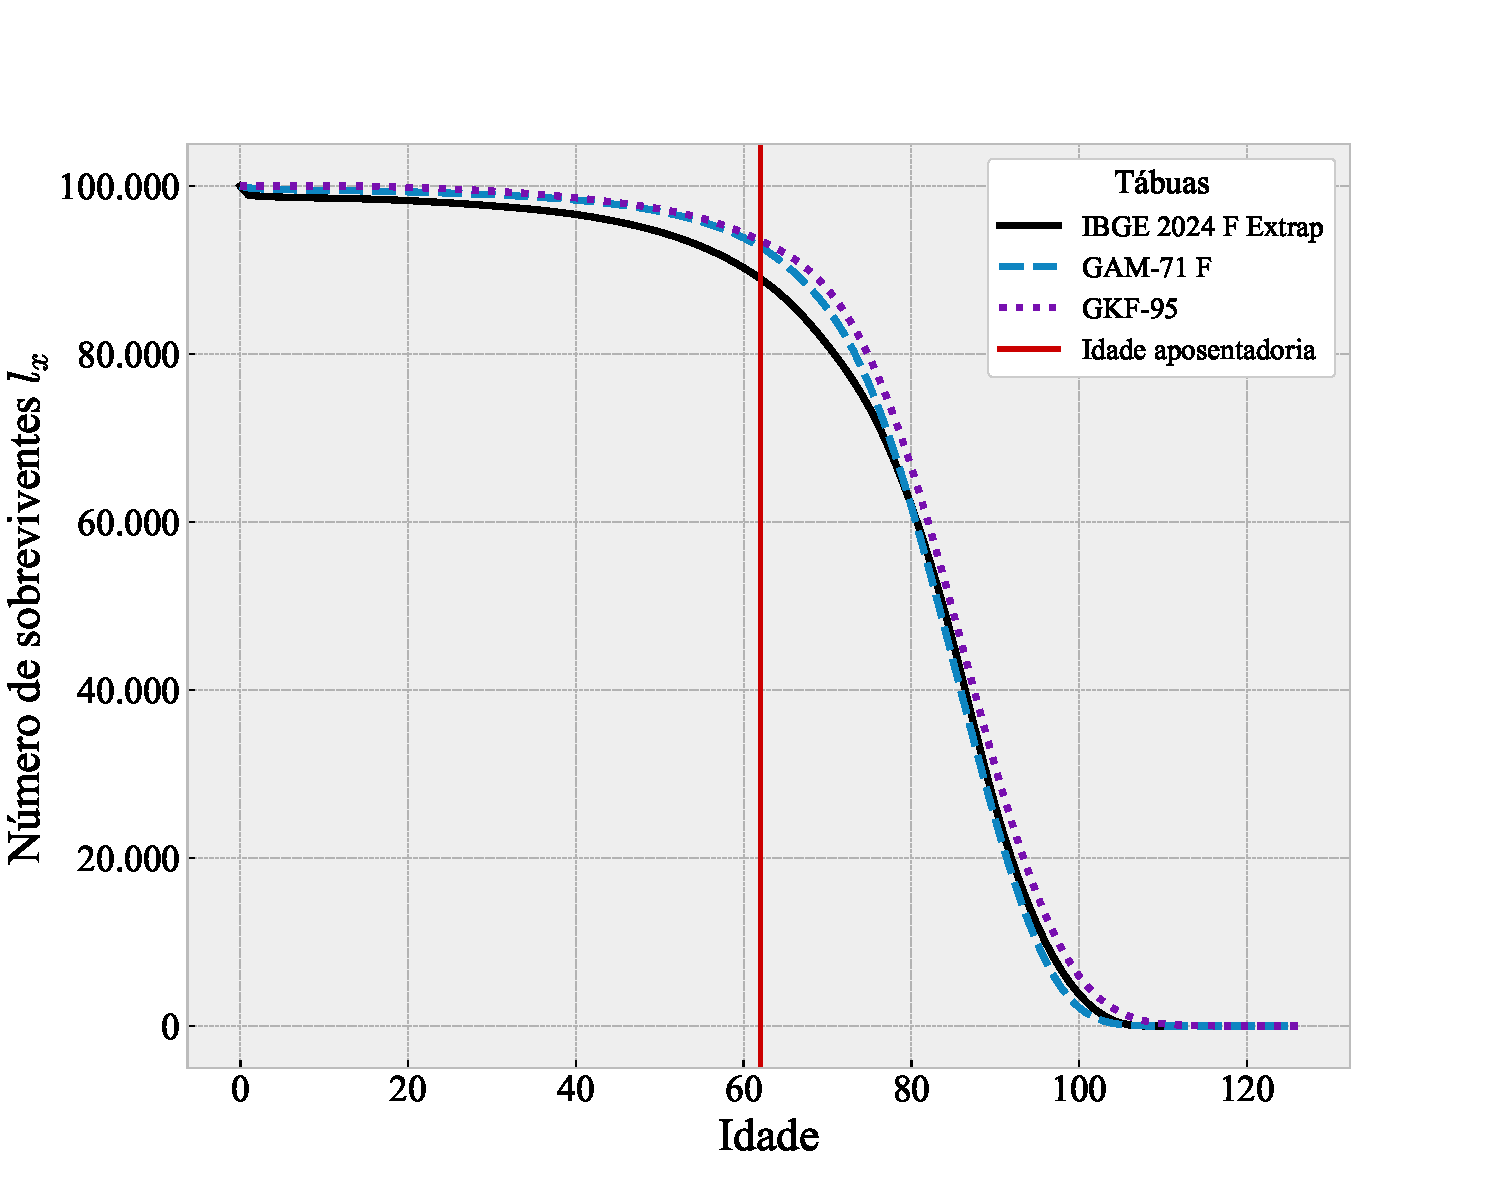
\includegraphics[width=0.9\textwidth, trim=0 0 0 2.5cm, clip]{curva_lx_fem.pdf}
            \end{figure}


    \end{frame}

    \begin{frame}
        \frametitle{Indicadores Exemplos}

        \begin{columns}

            \begin{column}{0.5\textwidth}
                \begin{itemize}
                    \item AT-55
                    \begin{itemize}
                        \item[$-$] $I_{Ativo} = 3,3$
                        \item[$-$] $I_{Aposentados} = -0,81$
                    \end{itemize}

                    \item BR-EMSmt 2015 M Agrav 25\%
                    \begin{itemize}
                        \item[$-$] $I_{Ativo} = 2,6$
                        \item[$-$] $I_{Aposentados} =  8,6$
                    \end{itemize}
                \end{itemize}
            \end{column}

            \begin{column}{0,5\textwidth}
                \begin{itemize}
                    \item GAM-71
                    \begin{itemize}
                        \item[$-$] $I_{Ativo} = 1,43$
                        \item[$-$] $I_{Aposentados} = 0,61$
                    \end{itemize}
                    
                    \item GKF 95
                    \begin{itemize}
                        \item[$-$] $I_{Ativo} = 1,89$
                        \item[$-$] $I_{Aposentados} =  9,04$
                    \end{itemize}
                \end{itemize}
            \end{column}

        \end{columns}

    \end{frame}

\section{Considerações}
    \begin{frame}
        \frametitle{Conclusões}
            \begin{itemize}
                \item Critério normativo pode ser insuficiente
                \item Possível vulnerabilidade normativa (Agravamento/Suavização)
                \item Estruturas etárias jovens, especialmente a do gênero masculino
                \item $I_{Ativo} > I_{Aposentados}$
            \end{itemize}
            
    \end{frame}

    \begin{frame}
        \frametitle{Limites e trabalhos futuros}
            \begin{itemize}
                \item[] Limites
                \begin{itemize}
                    \medskip
                    \item Distribuições simuladas
                    \medskip
                    \item Simplificação das variáveis
                    \medskip
                    \item Índice $I_F$ proposto
                \end{itemize}
                \medskip
                \item[] Trabalhos futuros
                \begin{itemize}
                    \medskip
                    \item Dados reais (mais de um benefício, variáveis reais)
                    \medskip
                    \item Múltiplos decrementos
                    \medskip
                    \item Aprimoramento do índice $I_F$
                    \medskip
                    \item Regulatório: Critérios baseados em métricas distribucionais (percentis)
                \end{itemize}
            \end{itemize}
            
    \end{frame}


%------------ Referências ------------%
\section{Referências}
    \begin{frame}[allowframebreaks]{Referências}
    
        \scriptsize
        Brasil. Portaria MTP nº 1.467, de 2 de junho de 2022. 2022. Diário Oficial da União.  
        
        \medskip
        
        Boyd, D. J.; Yin, Y. Public Pension Plan Demographics: Funding and Contribution Risk. Albany, NY, 2016.  
        
        \medskip
        
        Castro e Silva, L. G. d. Projeções dos Níveis e Padrões da Mortalidade no Brasil e Grandes Regiões 1950-2010-2110 pelo Método Coerente Lee-Carter Estendido e Outros: A Tábua BR Geracional e o Risco de Longevidade nas Instituições Previdenciárias do País. Tese (Tese de Doutorado) — Universidade Federal de Minas Gerais (UFMG), Belo Horizonte, 2019.
        
        \medskip
        
        Correa, C. S. Premissas atuariais em planos previdenciários: Uma abordagem atuarial e demográfica. [S.l.]: Appris Editora, 2018.  
        
        \medskip
        
        Rocha, A. S.; \textit{et al.}. Tábua de mortalidade de segurados válidos do regime próprio de previdência social do estado do Ceará.  
    
    \end{frame}

%------------ Fim ------------%
\section{Fim}
    \begin{frame}{Fim}
            \begin{center}
                \textbf{Obrigado!}
            \end{center}
    \end{frame}

\end{document}